\section{Description and Methodology}

This report describes three distinct systems for controlling LEDs on a game pad via user input; Each one more more refined than the last.

The first implementation is a simple polling-based approach. The second one uses interrupts, guaranteeing timely response to user input. The final system goes into stop mode, waking only when coerced to do so by an interrupt from the GPIO controller.

Energy consumption was noted for the polling- and sleep based versions of the system. The same repeat pattern of button presses were used in each of the measurements. This ensures easy comparison between the measurements.

As the interrupt-based system frequently sits noop-ing quietly by itself in a corner, its power usage is roughly equal to the polling-based version. It is therefore not considered in the results section. 

The system has been set up and tested with GDB.
When the system was to sleep in EM4 (see \ref{subsection:low-energy}), there was some confusion by the documentation provided for which registers to set. Diving into the depths of the GDB was deemed necessary.
Registers written to were examined by stepping through the program. The problem was found to lie with the values written to the registers, and not the registers themselves.

\subsection{Polling system}
\label{subsection:polling}

The initial system implements a simple polling-based mechanism for updating the LEDs on the game pad. The main loop simply loads whatever values are found on the game pad (GPIO port C, pins 0-7), shifts them to the appropriate position required by the output port (GPIO port A, pins 8 - 15), and sets the corresponding pins to logical low.

\begin{lstlisting}[caption={Polling loop}, label={lst:polling-loop}]
_reset:
    /* Boilerplate code omitted for readability */

    ldr r1, =GPIO_PA_BASE       /* Load PORT A register base address    */
    ldr r2, =GPIO_PC_BASE       /* Load PORT C register base address    */

    /* Main loop */
    LOOP:
        ldr r2, [r3, #GPIO_DIN] /* Load button values       */
        lsl r2, r2, #8          /* Shift values 0-7 to 8-15 */
        str r2, [r1, #GPIO_DOUT]/* Write to LED register    */
        bl LOOP

\end{lstlisting}

This naïve implementation is exceptionally good at eating all available power, a trait not desirable in what was supposed to be an energy efficient system. The main loop runs at all times, even when no update is needed, eating away at scarce energy resources.


\subsection{Interrupt system}

The second system contains a simple, yet important architectural change. The system no longer blindly loads register values each tick, instead updating only when receiving interrupts from GPIO port C.

A number of flags are set to allow for interrupt-driven event handling, as shown in the following code segment \ref{lst:interrupt-flags}.

Highlights include allowing for interrupt generation and -acceptance on GPIO port C, edge-driven interrupts on both hi-lo and lo-hi transitions from the game pad, as well as enabling both odd and even interrupts.

\lstinputlisting[caption={Interrupt flags}, label={lst:interrupt-flags}, linerange={113-125}]{../code/ex1.s}

Call back handlers (listing \ref{lst:register-interrupt-handlers}) are registered for both odd and even pins. These allow us to handle the interrupts generated by the game pad buttons.

\lstinputlisting[caption={Registering interrupt handlers}, label={lst:register-interrupt-handlers}, linerange={33-33, 43-43}]{../code/ex1.s}

The main loop is modified (listing \ref{lst:new-main-loop}) to halt execution until the call back handler has run. This is an important step towards reducing power consumption when idle.

\lstinputlisting[caption={New main loop}, label={lst:new-main-loop},linerange={132-133, 138-142}]{../code/ex1.s}

First order of the day for the interrupt handler (listing \ref{lst:interrupt-handler}) is clearing any potential lingering interrupts. This to avoid the interrupt handler being interrupted by another interrupt, hindering anything productive from being done.
Game pad output is then loaded from GPIO port C, stored, bit shifted to match the output pins on port A, and written to the registry.

Interrupts are available for both edge transitions on the game pad, with the attached handler executing on both events.
This ensured that the LEDs are updated on both button presses and releases. It contrasts with the earlier polling approach, where the values were blindly copied on each tick, regardless of the values changed or not.

\lstinputlisting[caption={Interrupt handler function}, label={lst:interrupt-handler}, linerange={151-156, 162-170}]{../code/ex1.s}

\subsection{Sleeping system}
\label{subsection:low-energy}

To save energy while running the program, it can use a low energy mode.
There are five different energy modes that can be used, with different peripherals available, as can be seen in figure \ref{fig:energy_modes}.\cite{referencemanual}

\begin{figure}[H]
\centering
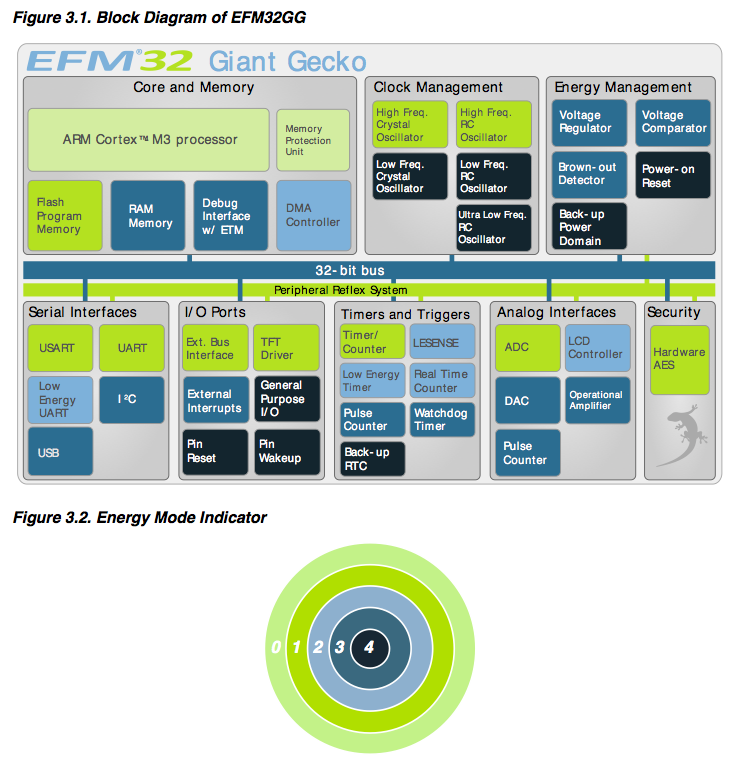
\includegraphics[scale=0.5]{figures/energymodes.png}
\caption{The different energy modes and available peripherals}
\label{fig:energy_modes}
\end{figure}

The trade off to use a low energy mode is that it takes some time to wake up (that is, to go from current energy mode to EM0)
From EM2 and EM3  the wake up time is about 2 $\mu$s, while in EM4 it is 160 $\mu$s. EM1 has no latency.
For the user, a 0.1 s latency would feel instantaneous.\cite{response}
This means that even EM4 is satisfactory for the application, as after waking up from this mode will feel fast.

The only thing that needs to be done while the application is sleeping, is to wait for interrupts on the GPIO ports.
This excludes EM4, as to wake up from this mode with interrupts is only supported on a small number of GPIO ports.

Thus the deepest sleep the application can use is EM3.

\lstinputlisting[caption={Sleep mode enabling},label={lst:sleep},linerange={127-130}]{../code/ex1.s}

In listing \ref{lst:sleep}, energy mode 3 is enabled when the wait for instruction (wfi) instruction is called, or the code returns from an interrupt.
The wfi instruction is called in listing \ref{lst:loop}, the main loop of the program. 
This means that each time the program returns from an interrupt, wfi is called and the program goes to sleep again.

\lstinputlisting[caption={Main loop}, label={lst:loop}, linerange={133-142}]{../code/ex1.s}

In addition, the code in listing \ref{lst:loop} also disables the output GPIO ports, as to prevent GPIO leakage.\cite{energy} 
These output ports are again enabled in the interrupt handler, before they are used to power the LEDs.

\subsubsection{Further improvements}

To get the application to sleep in EM4, a small hardware change would have to be done.
An idea would be to multiplex the signals from the buttons.
Every time a a button is pressed, a signal would go high.
This signal could go to one of the GPIO ports supported to wake the unit from EM4.
This could save a lot of energy, as a micro processor running in EM4 can use as little as 20nA.\cite{modes}
